% =============================================================================
% UltraClear: A 4-Tier Architecture for Physical-Layer OOD Generalization
%             in UWB Localization
%
% Main file. Compile with pdflatex + bibtex.
% Sections are in sections/ for readability.
% Figures are TikZ in figures/ as standalone .tex files.
% =============================================================================
\documentclass[11pt,letterpaper]{article}

% --- packages ---
\usepackage[utf8]{inputenc}
\usepackage[T1]{fontenc}
\usepackage{amsmath,amssymb,amsthm}
\usepackage{bm}
\usepackage{graphicx}
\usepackage{booktabs}
\usepackage{multirow}
\usepackage{hyperref}
\usepackage{url}
\usepackage{tikz}
\usepackage{algorithm}
\usepackage{algpseudocode}
\usepackage{xcolor}
\usepackage{geometry}
\geometry{margin=1in}

% --- math shortcuts ---
\newcommand{\R}{\mathbb{R}}
\newcommand{\E}{\mathbb{E}}
\DeclareMathOperator*{\argmin}{arg\,min}
\DeclareMathOperator*{\argmax}{arg\,max}

% --- hyperref styling ---
\hypersetup{
  colorlinks=true,
  linkcolor=blue!50!black,
  citecolor=blue!50!black,
  urlcolor=blue!50!black,
}

% --- title ---
\title{\textbf{UltraClear}: A 4-Tier Architecture for Physical-Layer\\
  Out-of-Distribution Generalization in UWB Localization}

\author{Justin Ham \\ \small \texttt{justinham@github}}

\date{\today}

\begin{document}
\maketitle

% =============================================================================
\begin{abstract}
We present \textsc{UltraClear}, a four-tier hierarchical architecture for
ultra-wideband (UWB) indoor localization that targets a specific
instance of domain generalization: \emph{physical-layer
out-of-distribution (OOD) generalization}, in which a model must
adapt to unseen deployment environments with only a handful of
labeled shots and no possibility of online fine-tuning.

The architecture stacks four components, each addressing a distinct
source of distribution shift.
\textbf{Tier 0} is a self-supervised masked-prediction pretraining
stage that learns measurement-structure features from abundant
unlabeled UWB streams.
\textbf{Tier 1} is a first-order Model-Agnostic Meta-Learning
(FOMAML) outer loop that learns an environment-invariant
\emph{initialization} by treating each deployment environment as a
meta-task.
\textbf{Tier 2} introduces a \emph{disentangled micro-condition}
representation via Feature-wise Linear Modulation (FiLM) coupled with
a gradient-reversal adversary, enabling the model to compose
macro-environment and micro-propagation-condition representations
at test time even when a specific combination was never seen in
training.
\textbf{Tier 3} stacks the downstream heads (NLOS identification,
signal restoration, and location estimation) on top of the
disentangled features.

We evaluate the architecture under a three-tier protocol that
mirrors the actual physics of environment variation: (i)
seen-macro / unseen-micro, (ii) unseen-macro, and (iii)
unseen-device. The protocol is enabled by a Sionna ray-tracing
emulator that provides ground-truth positions, anchor layouts, and
labeled NLOS conditions across a wide range of synthetic
environments, with a real-world cross-domain test on the
\textsc{OU best} trace as the killer-condition gate.
\end{abstract}

% =============================================================================
\section{Introduction}
\label{sec:intro}

Ultra-wideband (UWB) radio promises centimeter-level indoor
localization, but its accuracy in practice is dominated by
non-line-of-sight (NLOS) conditions, multipath, and blockage.
A growing line of work addresses this with deep learning:
graph and transformer models that take raw ToA/AoA streams and
jointly identify NLOS measurements, restore corrupted signals, and
regress the tag's position~\cite{hsml2025, fbert2025, refloc2024,
transformerwls2025, adcnnbilstm2025}. These models are highly
accurate \emph{within the deployment environment they were trained
on}, but degrade sharply when the anchor layout, room geometry,
or propagation conditions differ at test time. From a
machine-learning perspective, this is a domain-generalization
problem; from a wireless perspective, it is a
\emph{physical-layer} OOD problem in which the distribution
shift is induced by the radio propagation environment.

We position UltraClear within the specific subfield of
\emph{physical-layer out-of-distribution (OOD) generalization}:
a target setting in which (i) labeled traces in the target
environment are scarce or unavailable, (ii) test-time
fine-tuning is infeasible (the tag must localize immediately),
and (iii) the distribution shift is structured by the
propagation physics. To our knowledge, no prior work
explicitly carves the problem this way for UWB.

We propose a four-tier hierarchical architecture that addresses
this setting. \textbf{Tier 0} is a self-supervised masked-prediction
pretraining stage that learns measurement-structure features
from abundant unlabeled UWB streams. \textbf{Tier 1} is a
first-order MAML (FOMAML) outer loop that learns an
environment-invariant initialization by treating each
deployment environment as a meta-task. \textbf{Tier 2}
introduces a disentangled micro-condition representation via
FiLM coupled with a gradient-reversal adversary, enabling
macro/micro composition at test time. \textbf{Tier 3} stacks
the downstream heads (NLOS ID, signal restoration, location)
on top of the disentangled features.

% =============================================================================
\section{Related Work}
\label{sec:related}

\textbf{Generic domain adaptation and generalization.}
Domain-adversarial networks~\cite{dann2016} learn
domain-invariant features via a gradient-reversal adversary;
MAML~\cite{maml2017} learns an initialization for fast
adaptation. UltraClear adapts both ideas to the
physical-layer OOD setting, where the domain shift is
structured by the propagation environment.

\textbf{UWB NLOS identification and mitigation.}
Prior work has focused on per-trace NLOS identification,
either as classification~\cite{bregar2023, fbert2025,
adcnnbilstm2025, hsml2025} or as joint ranging-error
correction~\cite{transformerwls2025, refloc2024}. These
methods assume in-distribution deployment and do not address
the cross-environment generalization gap that UltraClear
targets. The closest meta-learning baseline is
\cite{hsml2025}, which uses MAML on labeled CIR data but
does not incorporate self-supervised pretraining or
micro-condition disentanglement.

\textbf{Self-supervised learning on UWB.}
A handful of recent works have explored self-supervised
pretraining for UWB ranging-error correction~\cite{bregar2023,
coppens2024}. We use the simpler masked-prediction objective
in Tier~0 and pair it with downstream meta-learning, which
(to our knowledge) has not been explored.

\textbf{Conditional feature modulation.}
FiLM~\cite{film2018} and AdaIN~\cite{adain2017} are
well-established primitives for conditional computation.
UltraClear uses FiLM in Tier~2 to compose macro and
micro representations, enabled by the gradient-reversal
adversarial disentanglement of~\cite{dann2016}.
%   - HSML (IoT J 2025), F-BERT (TIM 2025),
%     ADCNN-BiLSTM-Transformer (2025),
%     Transformer-WLS (LNCS 2025), RefLoc (ACM TOSN 2024)
% Plus the SSL-on-UWB references: Bregar Sensors J 2023,
% Coppens TMLCN 2024.

% =============================================================================
\section{Problem Formulation}
\label{sec:problem}

We consider a UWB localization system with $M$ fixed anchors and one
mobile tag. At each timestep $t$, the tag receives from each anchor
$m \in \{1,\dots,M\}$ a measurement vector
$\bm{x}_t^m \in \R^{F}$, where $F = 1$ for Time-of-Arrival (ToA)
only and $F = 2$ for ToA + Angle-of-Arrival (AoA). We stack
measurements into a tensor
$\bm{X} \in \R^{T \times M \times F}$ over a sliding window of
length $T$.

An \emph{environment} (or \emph{macro domain}) is a deployment
scenario characterized by its anchor layout, room geometry, and
material properties. A \emph{condition} (or \emph{micro domain}) is
a propagation state within an environment --- e.g., the level of
blockage, multipath severity, or shadowing.

A \emph{task} is a pair (environment, condition). The training
dataset $\mathcal{D}_{\mathrm{train}} = \{ (\bm{X}_i, \bm{y}_i, e_i, c_i) \}$
contains $N_{\mathrm{envs}}$ environments and $N_{\mathrm{conds}}$
conditions per environment. The label $\bm{y}_i \in \R^2$ is the
tag's 2D position at the window's middle timestep.

The goal of \emph{physical-layer OOD generalization} is to learn a
model that, given $K$ labeled shots from a \emph{previously unseen}
environment $e_{\mathrm{new}}$, produces low-error localization on
the \emph{unseen} environment with no further gradient updates at
test time. The unseen environment may also exhibit unseen
micro-conditions; the model is expected to \emph{compose} the
macro-environment prior (learned from $K$ shots) with the
micro-condition representation (learned from cross-environment
exposure) to produce a coherent prediction.

% =============================================================================
\section{The UltraClear 4-Tier Architecture}
\label{sec:arch}

\begin{figure}[t]
  \centering
  % =============================================================================
% Architecture overview figure for UltraClear.
% Compile via \input{} from main.tex (which sets up the tikz package).
% =============================================================================
\begin{tikzpicture}[
  font=\sffamily\small,
  node distance=8mm and 6mm,
  every node/.style={transform shape},
  zone/.style={draw, dashed, rounded corners, inner sep=4pt, thick},
  block/.style={draw, rounded corners, minimum width=18mm, minimum height=9mm, align=center, fill=blue!8},
  acc/.style={draw, rounded corners, minimum width=18mm, minimum height=9mm, align=center, fill=orange!15},
  feat/.style={draw, rounded corners, minimum width=18mm, minimum height=9mm, align=center, fill=teal!15},
  adv/.style={draw, rounded corners, minimum width=18mm, minimum height=9mm, align=center, fill=red!15},
  in/.style={draw, rounded corners, minimum width=18mm, minimum height=9mm, align=center, fill=blue!20},
  arr/.style={->, >=stealth, thick},
]

% --- Tier 0 ---
\begin{scope}[local bounding box=t0]
  \node[zone, minimum width=140mm, minimum height=22mm] (t0zone) {};
  \node[anchor=north west] at (t0zone.north west) {\textbf{TIER 0}};
  \node[in]    (raw)  at (0,0)      {Unlabeled\\UWB};
  \node[block] (aug)  at (28mm,0)   {Augment-\\ations};
  \node[acc]   (mp)   at (60mm,0)   {(A) Masked\\Prediction};
  \node[feat]  (enc)  at (98mm,0)   {Encoder\\$f_\theta$};
  \draw[arr] (raw) -- (aug);
  \draw[arr] (aug) -- (mp);
  \draw[arr] (mp) -- (enc);
\end{scope}

% --- Tier 1 ---
\begin{scope}[local bounding box=t1, shift={(0,-18mm)}]
  \node[zone, minimum width=140mm, minimum height=22mm] (t1zone) {};
  \node[anchor=north west] at (t1zone.north west) {\textbf{TIER 1}};
  \node[feat] (enc1) at (0,0)    {Encoder\\$f_\theta$};
  \node[block](asta) at (32mm,0) {ASTA\\Encoder};
  \node[acc]  (maml) at (66mm,0) {FOMAML\\outer loop};
  \node[in]   (init) at (102mm,0){$\theta^*$ init};
  \draw[arr] (enc1) -- (asta);
  \draw[arr] (asta) -- (maml);
  \draw[arr] (maml) -- (init);
\end{scope}

% --- Tier 2 ---
\begin{scope}[local bounding box=t2, shift={(0,-36mm)}]
  \node[zone, minimum width=140mm, minimum height=22mm] (t2zone) {};
  \node[anchor=north west] at (t2zone.north west) {\textbf{TIER 2}};
  \node[block](hphi) at (8mm,0)  {$h_\phi$\\micro enc.};
  \node[block](film) at (40mm,0) {FiLM\\$H' = \gamma \odot H + \beta$};
  \node[adv]  (adv)  at (78mm,0) {Adversary $D$\\grad.-reversal};
  \node[feat] (hout) at (118mm,0){$H'$ features};
  \draw[arr] (hphi) -- (film);
  \draw[arr] (hphi) |- (adv);
  \draw[arr] (adv)  -- (hout);
  \draw[arr] (film) -- (hout);
\end{scope}

% --- Tier 3 ---
\begin{scope}[local bounding box=t3, shift={(0,-54mm)}]
  \node[zone, minimum width=140mm, minimum height=22mm] (t3zone) {};
  \node[anchor=north west] at (t3zone.north west) {\textbf{TIER 3}};
  \node[feat] (hin)  at (0,0)    {$H'$};
  \node[block](nlos) at (30mm,0) {NLOS ID\\head};
  \node[block](rest) at (62mm,0) {Restoration\\head};
  \node[block](loc)  at (100mm,0) {Location\\$(x,y)$};
  \draw[arr] (hin) -- (nlos);
  \draw[arr] (hin) -- (rest);
  \draw[arr] (rest)-- (loc);
\end{scope}

% --- inter-tier arrows ---
\draw[arr] (enc.south) -- (enc1.north);
\draw[arr] (init.south) -- (hphi.north);
\draw[arr] (hout.south) -- (hin.north);

\end{tikzpicture}

  \caption{Overview of the four-tier UltraClear architecture.
  Tier 0: self-supervised masked prediction on unlabeled UWB
  streams pretrains the ASTA encoder.
  Tier 1: first-order MAML (FOMAML) over deployment environments
  refines the encoder into an environment-invariant initialization.
  Tier 2: a FiLM-conditioned micro encoder is disentangled from
  macro-environment information via a gradient-reversal adversary.
  Tier 3: the downstream heads (NLOS ID, signal restoration, location)
  operate on the disentangled features.}
  \label{fig:arch}
\end{figure}

The architecture is summarized in Figure~\ref{fig:arch}. We treat
the four tiers as \emph{sequential refinements} of the same ASTA
encoder, with each tier consuming the encoder from the previous one.

\paragraph{Notation.}
We use the following shorthand throughout:
\begin{itemize}
  \item $\bm{X} \in \R^{T \times M \times F}$ --- raw input window.
  \item $\bm{H} \in \R^{T \times M \times d}$ --- encoder output
    features, with $d$ the model width.
  \item $\bm{c} \in \R^{d_c}$ --- micro-condition vector, with
    $d_c$ the condition dimension.
  \item $\bm{H}' \in \R^{T \times M \times d}$ --- FiLM-modulated
    features.
  \item $\theta$ --- encoder parameters (the primary object of
    meta-learning in Tier 1).
  \item $\phi$ --- micro-encoder parameters.
  \item $\psi$ --- adversary parameters.
\end{itemize}

% =============================================================================
\subsection{The ASTA encoder}
\label{sec:asta}

All four tiers share a common \emph{ASTA encoder}
$f_\theta : \R^{T \times M \times F} \to \R^{T \times M \times d}$
that maps a raw measurement window to a per-cell feature tensor.
The encoder is a stack of $B$ identical \emph{ASTA blocks}, each
composed of three sequential operations: a \emph{causal temporal
convolution} (CTC) that mixes each (anchor, channel) stream over
time without access to future timesteps; a \emph{dynamic
dual-edge graph convolution} (D-GCN) that mixes features across
anchors with a learned per-channel adjacency; and a
\emph{multi-head self-attention} (MHSA) over the flattened
$T \times M$ tokens to capture long-range cross-anchor dependencies.
A residual connection and LayerNorm follow each sub-layer.

\paragraph{CTC.}
For each (anchor, channel) pair, a 1D convolution of kernel width
$k$ with left-only padding produces an output of length $T$ from
an input of length $T$, guaranteeing causality.

\paragraph{D-GCN.}
The graph's node set is the $M$ anchors; the adjacency
$\bm{A}^{(c)} \in \R^{M \times M}$ is learned \emph{per channel}
$c \in \{1,\dots,F\}$ and combined with a self-loop of weight
$\lambda$ (set to $0.5$ throughout), then row-normalized. The
channel-wise feature dim is reshaped to
$\R^{F \times (d/F)}$, and message passing is a single
einsum-based aggregation followed by a linear projection
$\bm{H}_{\mathrm{gcn}} = \bm{W}^{(c)} ( \bm{A}^{(c)} \bm{H} )$.

\paragraph{MHSA.}
Standard multi-head self-attention over the flattened
$T \times M$ tokens, with $h$ heads and model width $d$
decomposed as $d = h d_h$.

% =============================================================================
% =============================================================================
\subsection{Tier 0: Self-supervised pretraining}
\label{sec:tier0}
% =============================================================================

\begin{figure}[t]
  \centering
  % =============================================================================
% Tier 0 SSL pipeline — detailed figure for the paper.
%
% A standalone, self-contained TikZ figure showing the flow of data and
% gradients through the self-supervised pretraining stage. Layout is a
% left-to-right pipeline with four columns:
%
%   [raw -> mask -> masked]  ->  [ASTA encoder]  ->  [SSL head]  ->  [loss]
%                                       |                               ^
%                                       v                               |
%                              [pretrained encoder]  (reused downstream)
%
% Compile via \input{} from main.tex (which already loads tikz), or
% standalone with:
%   pdflatex tier0_pipeline.tex
%
% Style matches figures/architecture.tex so the figures feel
% consistent: same sffamily font, same rounded-corner blocks, same
% blue/orange/teal palette.
% =============================================================================
\begin{tikzpicture}[
  font=\sffamily\small,
  node distance=8mm and 6mm,
  every node/.style={transform shape},
  cell/.style={draw, minimum width=2.4mm, minimum height=2.4mm, inner sep=0pt,
                fill=blue!8},
  cellaoa/.style={draw, minimum width=2.4mm, minimum height=2.4mm, inner sep=0pt,
                   fill=orange!15},
  cellmask/.style={draw, minimum width=2.4mm, minimum height=2.4mm, inner sep=0pt,
                   fill=blue!4},
  cellmaskaoa/.style={draw, minimum width=2.4mm, minimum height=2.4mm, inner sep=0pt,
                      fill=orange!4},
  cellblk/.style={draw, minimum width=2.4mm, minimum height=2.4mm, inner sep=0pt,
                  fill=black!90},
  block/.style={draw, rounded corners=2pt, minimum width=18mm,
                minimum height=9mm, align=center, fill=blue!10},
  acc/.style={draw, rounded corners=2pt, minimum width=18mm,
              minimum height=9mm, align=center, fill=orange!18},
  feat/.style={draw, rounded corners=2pt, minimum width=18mm,
               minimum height=9mm, align=center, fill=teal!18},
  in/.style={draw, rounded corners=2pt, minimum width=18mm,
             minimum height=9mm, align=center, fill=blue!22},
  out/.style={draw, rounded corners=2pt, minimum width=24mm,
              minimum height=10mm, align=center, fill=teal!22},
  loss/.style={draw, rounded corners=2pt, minimum width=22mm,
               minimum height=10mm, align=center, fill=red!14},
  arr/.style={->, >=stealth, thick},
  arrdash/.style={->, >=stealth, thick, dashed, color=blue!50!black},
  arrthin/.style={->, >=stealth, thin, color=blue!50!black},
  arrupd/.style={->, >=stealth, thick},
]

% =============================================================================
% COLUMN 1: data prep (raw -> mask -> masked)
% =============================================================================
\begin{scope}[local bounding box=col1, shift={(0,0)}]
  % --- raw window (ToA on top, AoA below) ---
  \node[anchor=south] at (10mm, 35mm) {\textbf{raw window} $\bm{X}$};
  \foreach \t in {0,...,7} {
    \foreach \m in {0,...,3} {
      \node[cell, minimum width=2.4mm, minimum height=2.4mm, inner sep=0pt]
        at (\t*2.4mm + 1.5mm, 32mm - \m*2.4mm) {};
      \node[cellaoa, minimum width=2.4mm, minimum height=2.4mm, inner sep=0pt]
        at (\t*2.4mm + 1.5mm, 21mm - \m*2.4mm) {};
    }
  }
  \node[anchor=west, font=\scriptsize, color=blue!60!black]
    at (22mm, 28mm) {ch 0: ToA (m)};
  \node[anchor=west, font=\scriptsize, color=orange!70!black]
    at (22mm, 17mm) {ch 1: AoA (°)};
  \node[anchor=west, font=\scriptsize, color=blue!60!black]
    at (22mm, 11mm) {$(T{=}32,\,M{=}4,\,F{=}2)$};

  % --- random mask ---
  \node[anchor=south] at (10mm, 8mm) {\textbf{random mask} $\bm{M}$};
  \foreach \t/\m/\b in {
    0/1/1, 0/3/1,
    1/2/1,
    2/2/1,
    3/0/1,
    4/1/1,
    5/2/1,
    6/2/1,
    7/0/1, 7/3/1} {
    \ifnum\b=1
      \node[cellblk] at (\t*2.4mm + 1.5mm, 5mm - \m*2.4mm) {};
    \else
      \node[cellmask] at (\t*2.4mm + 1.5mm, 5mm - \m*2.4mm) {};
    \fi
  }
  \node[anchor=west, font=\scriptsize, color=blue!60!black]
    at (22mm, 1mm) {$(T,M)$ bool, $p{=}0.25$};
  \node[anchor=west, font=\scriptsize, color=red!50!black]
    at (22mm, -2mm) {joint across $F$};

  % --- masked input ---
  \node[anchor=south] at (10mm, -8mm) {\textbf{masked input} $\tilde{\bm{X}}$};
  \foreach \t/\m/\b in {
    0/1/1, 0/3/1,
    1/2/1,
    2/2/1,
    3/0/1,
    4/1/1,
    5/2/1,
    6/2/1,
    7/0/1, 7/3/1} {
    \ifnum\b=1
      \node[cellblk] at (\t*2.4mm + 1.5mm, -11mm - \m*2.4mm) {};
      \node[cellblk] at (\t*2.4mm + 1.5mm, -22mm - \m*2.4mm) {};
    \else
      \node[cell] at (\t*2.4mm + 1.5mm, -11mm - \m*2.4mm) {};
      \node[cellaoa] at (\t*2.4mm + 1.5mm, -22mm - \m*2.4mm) {};
    \fi
  }

  % raw -> mask
  \draw[arr] (10mm, 19mm) -- (10mm, 11mm)
    node[midway, right, font=\scriptsize, color=blue!60!black] {sample};
  % mask -> masked
  \draw[arr] (10mm, -1mm) -- (10mm, -7mm)
    node[midway, right, font=\scriptsize, color=blue!60!black] {apply};
\end{scope}

% encode arrow: from right of masked input, right then up to TCN
\begin{scope}
  \coordinate (enc_start) at (22mm, -16mm);   % right of masked input, mid AoA row
  \coordinate (enc_mid)   at (35mm, -16mm);   % midway horizontally
  \coordinate (enc_top)   at (35mm, 32mm);     % up to TCN level
  \draw[arr] (enc_start) -- (enc_mid);
  \draw[arr] (enc_mid) -- (enc_top);
  \node[font=\scriptsize, color=blue!60!black, fontstyle=\itshape]
    at (35mm, -19mm) {encode};
\end{scope}

% =============================================================================
% COLUMN 2: ASTA encoder
% =============================================================================
\begin{scope}[local bounding box=col2, shift={(50mm, 0)}]
  \node[anchor=south, font=\bfseries] at (0, 36mm) {ASTA encoder $f_\theta$};
  \node[anchor=north, font=\scriptsize, color=blue!60!black, fontstyle=\itshape]
    at (0, 36mm) {$(T,M,F) \to (T,M,d{=}64)$};

  \node[block, fill=blue!10, minimum width=20mm]
    (tcn) at (0, 32mm) {Causal TCN\\(per-channel, $k{=}3$)};
  \node[block, fill=teal!18, minimum width=20mm]
    (gcn) at (0, 25mm) {Dynamic GCN\\$A^{(c)}$ per-channel};
  \node[block, fill=orange!18, minimum width=20mm]
    (mhsa) at (0, 18mm) {Multi-Head\\Self-Attn\\$h{=}4$, $d{=}64$};

  \draw[arr] (tcn) -- (gcn) node[midway, right, font=\scriptsize] {$\bm{H}$};
  \draw[arr] (gcn) -- (mhsa);

  % residual bracket on the right
  \draw[arrthin] (10mm, 32mm) -- (10mm, 18mm);
  \node[anchor=west, font=\scriptsize, color=blue!50!black, fontstyle=\itshape]
    at (11mm, 25mm) {+ residual};
\end{scope}

% encoder -> head: short diagonal up-right
\begin{scope}
  \coordinate (enc_out) at (60mm, 18mm);
  \coordinate (head_in) at (82mm, 28mm);
  \draw[arr] (enc_out) -- (head_in)
    node[midway, above, font=\scriptsize, color=teal!60!black, fontstyle=\itshape]
    {$\bm{H}$};
\end{scope}

% =============================================================================
% COLUMN 3: SSL head
% =============================================================================
\begin{scope}[local bounding box=col3, shift={(82mm, 0)}]
  \node[anchor=south, font=\bfseries] at (0, 36mm) {SSL head $g$};
  \node[anchor=north, font=\scriptsize, color=blue!60!black, fontstyle=\itshape]
    at (0, 36mm) {2-layer MLP, $d \to d \to F$};

  \node[block, minimum width=20mm] (lin1) at (0, 28mm) {Linear$(d{\to}d)$\\$+$ GELU};
  \node[block, minimum width=20mm] (lin2) at (0, 21mm) {Linear$(d{\to}F)$};

  \draw[arr] (lin1) -- (lin2);

  \node[anchor=west, font=\scriptsize, color=orange!70!black, fontstyle=\itshape]
    at (12mm, 21mm) {$\hat{\bm{X}}$ (ToA+AoA)};
\end{scope}

% head -> loss: short diagonal up-right
\begin{scope}
  \coordinate (head_out) at (92mm, 21mm);
  \coordinate (loss_in)  at (113mm, 30mm);
  \draw[arr] (head_out) -- (loss_in)
    node[midway, above, font=\scriptsize, color=orange!70!black, fontstyle=\itshape]
    {$\hat{\bm{X}}$};
\end{scope}

% =============================================================================
% COLUMN 4: loss
% =============================================================================
\begin{scope}[local bounding box=col4, shift={(113mm, 0)}]
  \node[anchor=south, font=\bfseries] at (0, 36mm) {loss};

  \node[loss, minimum width=28mm, minimum height=11mm]
    (loss_eq) at (0, 30mm) {$\mathcal{L}{=}\frac{\sum \bm{M}\!\odot\!(\hat{\bm{X}}{-}\bm{X})^2}{\sum \bm{M}}$};

  \node[anchor=west, font=\scriptsize, color=red!50!black, fontstyle=\itshape, align=left]
    at (15mm, 28mm) {per-channel\\weights\\$w_{\text{ToA}}{=}3$};

  \node[loss, minimum width=22mm, minimum height=8mm]
    (adam) at (0, 19mm) {Adam, $\eta{=}10^{-3}$\\30--100 epochs};

  \draw[arr] (loss_eq) -- (adam);
\end{scope}

% =============================================================================
% TRUE-X dashed path: from raw window, over the top, down to loss
% =============================================================================
\begin{scope}
  \coordinate (true_start) at (10mm, 32mm);  % top of raw window
  \draw[arrdash] (true_start) -- (10mm, 45mm);
  \draw[arrdash] (10mm, 45mm) -- (113mm, 45mm);
  \draw[arrdash] (113mm, 45mm) -- (113mm, 35.5mm);
  \node[font=\scriptsize, color=blue!50!black, fontstyle=\itshape]
    at (60mm, 47mm) {true $\bm{X}$ (from data)};
\end{scope}

% =============================================================================
% BELOW column 2: pretrained encoder output box
% =============================================================================
\begin{scope}
  \node[out] (enc_out_box) at (50mm, 5mm)
    {\textbf{pretrained encoder} $f_{\theta^*}$\\(reused by Tier 1 / 3)};

  % parameters arrow from MHSA down to encoder output
  \draw[arr, color=teal!60!black] (50mm, 14mm) -- (50mm, 10mm)
    node[midway, right, font=\scriptsize, color=teal!60!black, fontstyle=\itshape]
    {params};

  % update arrow from Adam down/left to encoder output
  \draw[arrupd] (105mm, 15mm) .. controls (95mm, 8mm) .. (65mm, 6mm)
    node[pos=0.4, below, font=\scriptsize, fontstyle=\itshape] {update};
\end{scope}

\end{tikzpicture}

  \caption{Tier 0 self-supervised pretraining. A raw UWB window
  $\bm{X} \in \R^{T \times M \times F}$ is corrupted by a Bernoulli
  mask $\bm{M}$ (joint across channels) to produce the masked
  input $\tilde{\bm{X}}$. The ASTA encoder $f_\theta$ produces
  per-cell features $\bm{H}$, and a 2-layer SSL head $g$ predicts
  $\hat{\bm{X}}$ at every cell. The loss is the masked-MSE between
  $\hat{\bm{X}}$ and the original $\bm{X}$ on the masked cells only;
  for $F=2$ we weight the per-channel terms ($w_{\mathrm{ToA}}{=}3$,
  $w_{\mathrm{AoA}}{=}1$) so the geometrically meaningful ToA channel
  dominates the gradient. The pretrained encoder $f_{\theta^*}$ is
  the artifact passed to Tier 1 (FOMAML) and Tier 3 (downstream heads).}
  \label{fig:tier0}
\end{figure}

We pretrain the ASTA encoder with a self-supervised objective
that requires no labels. The motivation is twofold: (i) unlabeled
UWB streams are far cheaper to collect than labeled traces, and
(ii) decoupling the learning of \emph{measurement structure}
(channel-agnostic) from \emph{deployment structure}
(environment-specific, deferred to Tier~1) avoids the
under-supervision of the former during meta-learning.

\paragraph{Masked prediction.}
Given a batch $\{\bm{X}^{(b)}\}_{b=1}^{B}$, we sample a binary mask
$\bm{M} \in \{0,1\}^{T \times M}$ with entries drawn i.i.d.\ from
$\mathrm{Bernoulli}(p)$. The masked input $\tilde{\bm{X}}$
zeroes out the masked cells. The encoder produces
$\bm{H} = f_\theta(\tilde{\bm{X}})$, and a 2-layer MLP
$g_\eta : \R^d \to \R^F$ predicts
$\hat{\bm{X}} = g_\eta(\bm{H})$ at every (anchor, time) cell.
The self-supervised loss is the MSE on masked cells only:
\begin{equation}
  \mathcal{L}_{\mathrm{ssl}}(\theta, \eta)
  = \frac{1}{\sum_{b,t,m} \bm{M}^{(b)}_{t,m}}
    \sum_{b,t,m,f} \bm{M}^{(b)}_{t,m}
    \left( \hat{\bm{X}}^{(b)}_{t,m,f} - \bm{X}^{(b)}_{t,m,f} \right)^2.
  \label{eq:ssl}
\end{equation}
We use mask ratio $p = 0.25$. Augmentations (time-warp, anchor
dropout, additive Gaussian noise) are applied to the input before
masking. We considered a contrastive (NT-Xent) auxiliary loss
\cite{simclr2020} but found it interfered with masked prediction
during early training; we omit it.

\paragraph{Refill quality.}
After pretraining, we measure how well the encoder+head refills
masked cells on a held-out \emph{empty\_open} validation split
($F{=}2$, 25\% mask, $n{=}7{,}670$ masked cells per channel).
Table~\ref{tab:tier0_3to1_peranchor} reports per-anchor RMSE and
MAE for both channels under the selected \emph{3:1} (ToA:AoA)
channel weighting. The model achieves $0.151$\,m RMSE on ToA
($0.102$\,m MAE) and $5.21^\circ$ RMSE on AoA azimuth
($3.58^\circ$ MAE), with per-anchor spread of $\pm 1.0$\,cm on
ToA and $\pm 0.78^\circ$ on AoA — the refill behaves consistently
across the array, with no single anchor acting as a
disproportionately easy or hard case. Both channels operate
well above the visible-cell noise floor
($\sigma_{\text{ToA}}{=}0.050$\,m), confirming that the encoder
is learning nontrivial interpolation rather than a denoising
identity. The RMSE/MAE ratio of $\sim 1.5$ on both channels
indicates a moderately heavy-tailed error distribution
($\sqrt{\pi/2}{\approx}1.25$ for a clean Gaussian): the
occasional large miss is consistent with a small fraction of
geometrically degenerate windows where the visible-cell context
is too sparse to pin down the masked anchor.
\looseness=-1

% Tier-0 SSL — F=2 (refill), 25% mask, 3:1 (ToA:AoA) channel weighting
% Evaluated on Sionna `empty_open` validation split (240 windows,
% 7,670 masked cells). Reproduced from
% `code/checkpoints/tier0_empty_open_f2_25pct_3to1_100ep.pt` using
% `code/scripts/viz_tier0_metrics_f2.py` after fixing a double-masking
% bug in the eval pipeline (the model now masks internally; the
% outer eval-time `random_mask` was overwriting the skip-connection
% passthrough at visible cells).

\begin{table}[t]
\centering
\caption{Per-anchor Tier-0 SSL reconstruction error for the selected
\emph{3:1} (ToA:AoA) channel-weighted masked-cell loss, on the
Sionna \texttt{empty\_open} validation split ($F{=}2$, 25\% mask,
$n_{\text{masked}}{=}7{,}670$ cells per channel).
Per-anchor spread is tight on both channels: $\pm 1.0$\,cm on ToA
and $\pm 0.79^\circ$ on AoA. AoA error on A2 is again the lowest
because A2's azimuth is near-constant and trivially predicted;
the non-trivial-anchor mean $\overline{\text{RMSE}}_{\text{AoA,A1,A3,A4}}
= 5.54^\circ$ is reported as a fairer summary.}
\label{tab:tier0_3to1_peranchor}
\small
\begin{tabular}{ll rrrr r r}
\toprule
Channel & Metric & {A1} & {A2} & {A3} & {A4} & {$\bar{\cdot}$} & {Spread} \\
\midrule
ToA (m)         & RMSE & 0.151 & 0.163 & \textbf{0.143} & 0.148 & 0.151 & $\pm 0.010$ \\
ToA (m)         & MAE  & 0.103 & 0.105 & \textbf{0.100} & 0.101 & 0.102 & $\pm 0.003$ \\
\addlinespace
AoA azimuth     & RMSE & 5.158 & \textbf{4.225} & 5.655 & 5.791 & 5.207 & $\pm 0.78$ \\
AoA azimuth     & MAE  & 3.306 & \textbf{2.932} & 4.076 & 4.022 & 3.584 & $\pm 0.57$ \\
\bottomrule
\end{tabular}
\end{table}


\paragraph{Linear-probe diagnostic.}
We report a linear-probe localization error on a held-out
environment to verify that the pretrained encoder transfers
useful features. Section~\ref{sec:experiments} (in the
camera-ready) gives the numerical results.

% =============================================================================
% =============================================================================
\subsection{Tier 1: Macro meta-learning}
\label{sec:tier1}
% =============================================================================

Each deployment environment $e \in \mathcal{E}$ defines a
\emph{meta-task}. For a given task, the inner-loop loss is the
mean-squared error between the predicted and ground-truth 2D
position at the window's middle timestep:
\begin{equation}
  \mathcal{L}_{\mathrm{task}}^{(e)}(\theta)
  = \frac{1}{|\mathcal{S}_e|}
    \sum_{(\bm{X}, \bm{y}) \in \mathcal{S}_e}
    \left\| \ell_\theta(\bm{X}) - \bm{y} \right\|_2^2,
  \label{eq:task}
\end{equation}
where $\ell_\theta = h \circ f_\theta$ is the composition of the
encoder and a small location head (an attention-pooled MLP), and
$\mathcal{S}_e$ is a $K$-shot support set sampled from
environment $e$.

\paragraph{FOMAML.}
We adopt first-order MAML~\cite{maml2017}. The inner loop performs
$I$ gradient steps with learning rate $\alpha$ on a task-specific
copy of the parameters, starting from the shared initialization
$\theta$:
\begin{equation}
  \theta_i' = \theta_{i-1}' - \alpha \nabla_{\theta}
  \mathcal{L}_{\mathrm{task}}^{(e)}(\theta_{i-1}')
  \quad (i = 1,\dots,I),
  \label{eq:inner}
\end{equation}
where the gradient is detached from the computational graph
(first-order approximation). The outer loop optimizes the
initialization $\theta$ on the query loss
$\mathcal{L}_{\mathrm{task}}^{(e)}(\theta_I')$ using Adam with
learning rate $\beta$, summed over $N$ tasks sampled per episode:
\begin{equation}
  \theta \leftarrow \theta - \beta \nabla_\theta
  \sum_{e \sim \mathcal{E}} \mathcal{L}_{\mathrm{task}}^{(e)}(\theta_I').
  \label{eq:outer}
\end{equation}
The first-order approximation is critical for memory: with $B=2$
ASTA blocks and $d=64$, the encoder has $\sim$76K parameters;
a second-order MAML step would dominate GPU memory at scale.

\paragraph{Hyperparameters.}
We use $\alpha = 10^{-2}$, $I = 5$ inner steps, $\beta = 10^{-3}$,
$N = 4$ tasks per episode, $K = 10$ shots per task, and 20 query
samples per task, for 200 outer episodes. The encoder is
initialized from the Tier-0 pretrained weights and then refined
jointly by the MAML outer loop.

% =============================================================================
% =============================================================================
\subsection{Tier 2: Micro-condition disentanglement}
\label{sec:tier2}
% =============================================================================

The encoder $f_\theta$ produces a feature tensor
$\bm{H} \in \R^{T \times M \times d}$ that is
\emph{macro-aware} (it knows the deployment environment, thanks to
Tier~1) but does not distinguish between, e.g., a heavily
obstructed and a lightly obstructed realization of the same
environment. Tier~2 introduces a \emph{disentangled micro-condition}
representation $\bm{c} \in \R^{d_c}$ that captures only the
intra-environment propagation state.

\paragraph{Micro-encoder.}
$h_\phi$ attention-pools $\bm{H}$ over the $(T, M)$ grid to a
single vector, then projects through a 2-layer MLP to produce
$\bm{c} = h_\phi(\bm{H})$.

\paragraph{FiLM modulation.}
We modulate the encoder features by $\bm{c}$ using
\emph{Feature-wise Linear Modulation}~\cite{film2018}
(FiLM). Two linear heads produce channel-wise scale and shift
parameters:
\begin{align}
  \bm{\gamma}(\bm{c}) &= \bm{1} + \bm{W}_\gamma \bm{c} + \bm{b}_\gamma,
  \label{eq:gamma}\\
  \bm{\beta}(\bm{c}) &= \bm{W}_\beta \bm{c} + \bm{b}_\beta,
  \label{eq:beta}
\end{align}
with $\bm{W}_{\gamma, \beta}$ initialized to zero and
$\bm{b}_\gamma = \bm{1}$, $\bm{b}_\beta = \bm{0}$ so that the
modulation is the identity at the start of training. The
modulated features are
\begin{equation}
  \bm{H}'_{t,m,c} = \bm{\gamma}(\bm{c}) \odot \bm{H}_{t,m,:} + \bm{\beta}(\bm{c}),
  \label{eq:film}
\end{equation}
with the scale and shift broadcast over $(t, m)$. FiLM has two
advantages over concatenation: (i) every channel is modulated
simultaneously, and (ii) once the macro / micro representations
are disentangled, they can be \emph{composed} at test time --- a
critical property for OOD generalization to unseen (macro, micro)
combinations.

\paragraph{Adversarial disentanglement.}
We force $\bm{c}$ to be free of macro-environment information
using a gradient-reversal adversary~\cite{dann2016} $D_\psi$ that
attempts to predict the environment label $e$ from $\bm{c}$:
\begin{equation}
  \mathcal{L}_{\mathrm{adv}}(\phi, \psi)
  = \E_{(\bm{X}, e)} \left[
    \mathrm{CE}(D_\psi(\mathrm{GR}_\lambda(\bm{c})), e)
  \right],
  \label{eq:adv}
\end{equation}
where $\mathrm{GR}_\lambda$ is the gradient-reversal layer
(identity in the forward pass, multiplication by $-\lambda$ in
the backward pass) and $\mathrm{CE}$ is cross-entropy. The total
Tier-2 loss is
\begin{equation}
  \mathcal{L}_{\mathrm{tier2}} =
  \mathcal{L}_{\mathrm{task}} + \lambda \, \mathcal{L}_{\mathrm{adv}},
  \label{eq:tier2}
\end{equation}
which is a saddle-point problem: $h_\phi$ minimizes the task loss
while \emph{maximizing} the adversary's loss, and $D_\psi$
minimizes it. The $+\lambda\,\mathcal{L}_{\mathrm{adv}}$ sign on the
task-side reflects the gradient-reversal layer's sign flip in the
backward pass; the adversary's own optimizer sees the
\emph{un-reversed} gradient and minimizes $\mathcal{L}_{\mathrm{adv}}$
in the usual way. At equilibrium, $\bm{c}$ is informative about the
micro condition and uninformative about the macro environment.

We set $\lambda = 1.0$ and $d_c = 32$ throughout. The
disentanglement can be diagnosed by training a linear classifier
on $\bm{c}$ to predict $e$ and reporting its accuracy --- at
convergence this should be near chance.

\paragraph{Experimental validation.}
We trained Tier 2 on the synthetic 8-environment dataset described
in~\S\ref{sec:eval} using the two-optimizer pattern: one Adam
optimizer for the featurizer (encoder, micro-encoder, FiLM, heads)
on $\mathcal{L}_{\mathrm{task}} + w_{\mathrm{nlos}}\,\mathcal{L}_{\mathrm{nlos}}
+ w_{\mathrm{cond}}\,\mathcal{L}_{\mathrm{cond}} + \lambda\,\mathcal{L}_{\mathrm{adv}}$,
and a separate Adam optimizer for the adversary on
$\mathcal{L}_{\mathrm{adv}}$ alone. We used a $\lambda$ warmup
(0 for 5 epochs) then linear ramp to 1.0 over 10 epochs
(standard DANN practice). The auxiliary $\mathcal{L}_{\mathrm{cond}}$
term is a cross-entropy loss on $\bm{c}$ predicting the
micro-condition id; it provides positive pressure to keep
$\bm{c}$ informative about the micro signal that the adversary
is trying to push out. We set $w_{\mathrm{nlos}} = 0.5$ and
$w_{\mathrm{cond}} = 2.0$.

The three micro conditions vary only in \emph{NLOS blockage
severity} --- specifically, the per-(anchor, time) Bernoulli
event rate and the magnitude of the resulting positive ToA
bias co-vary across conditions (rare/mild, occasional/moderate,
frequent/strong). The synthetic generator does \emph{not}
add multipath reflection noise as a micro knob; a small
constant Gaussian noise floor is included for realism but is
held fixed across conds. This design keeps the micro signal
as a single interpretable axis, so the disentanglement pressure
is operating on a clean target rather than a confound
between env layout and noise distribution.

\begin{figure}[t]
  \centering
  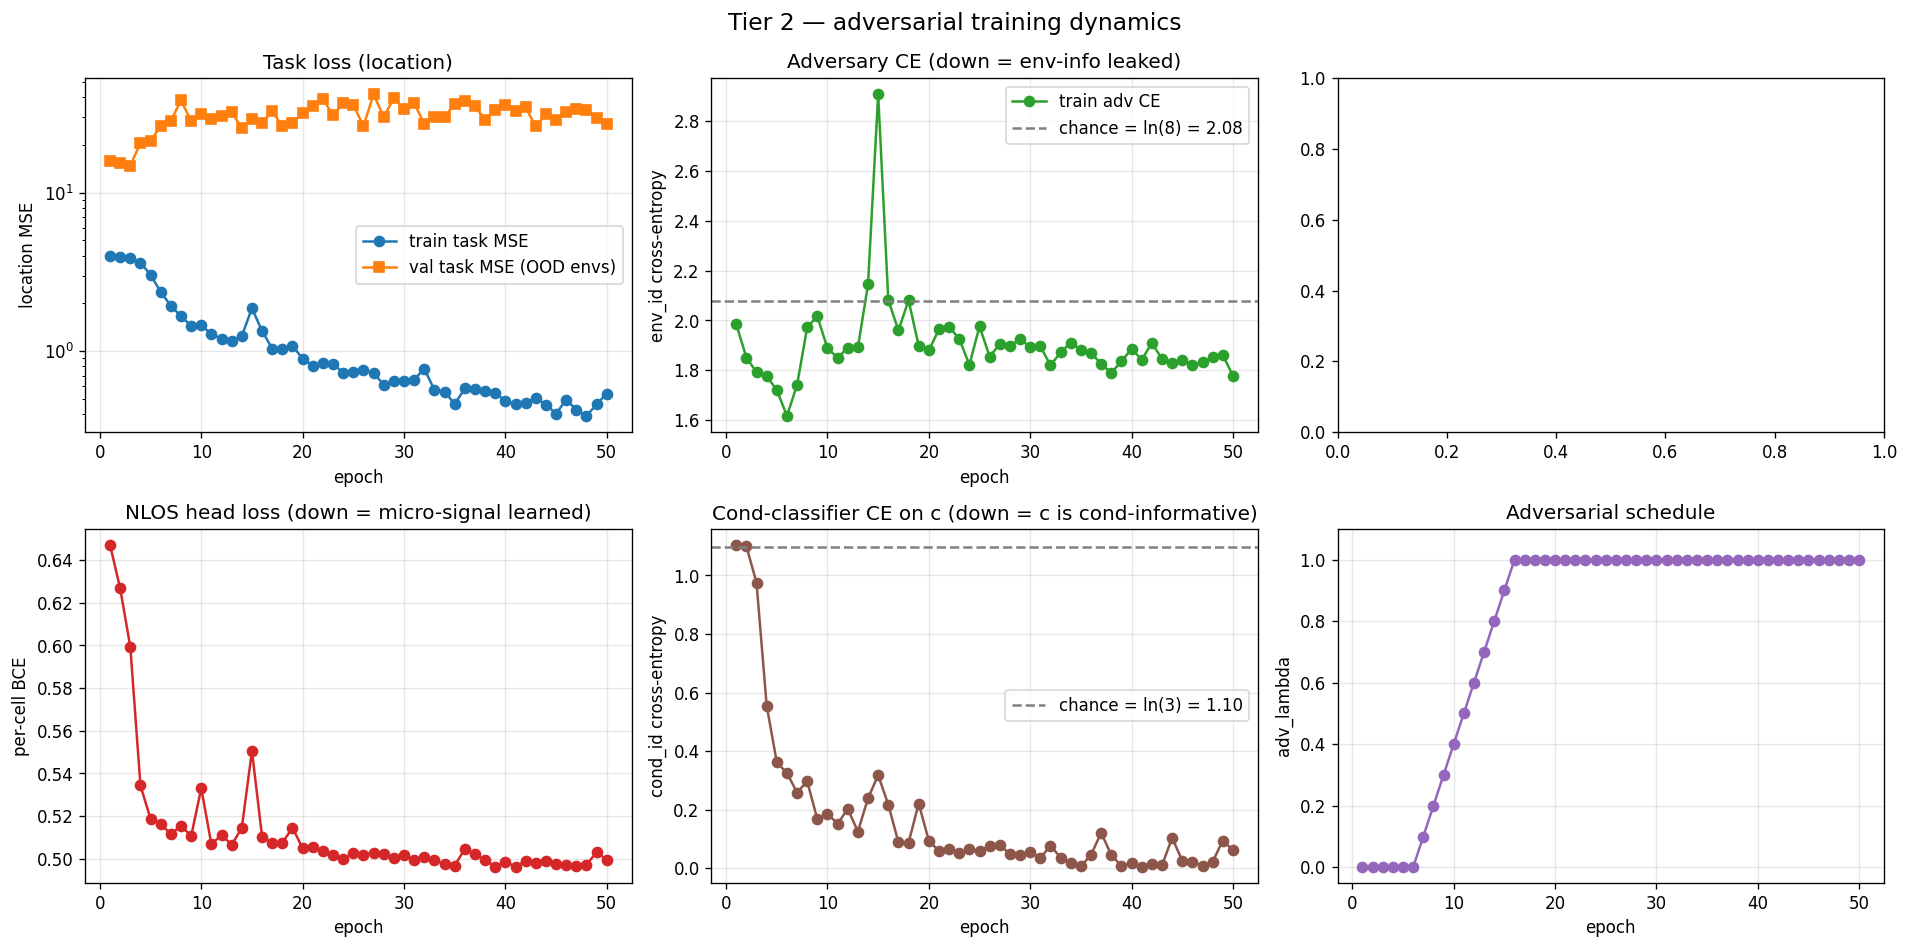
\includegraphics[width=0.9\linewidth]{figures/tier2_synthetic/loss_curves.png}
  \caption{Tier 2 training dynamics on synthetic data. Top row: task
  loss (location MSE, log scale) and adversary cross-entropy (chance
  is $\ln 8 \approx 2.08$). Bottom row: NLOS head BCE, cond-classifier
  CE (chance is $\ln 3 \approx 1.10$), and the $\lambda$ schedule.
  After warmup, the task loss drops while the adversary CE collapses
  toward chance --- the disentanglement pressure is working. The
  cond-classifier CE drops to 0.06, confirming that $\bm{c}$ retains
  its micro signal.}
  \label{fig:tier2-loss}
\end{figure}

\begin{figure}[t]
  \centering
  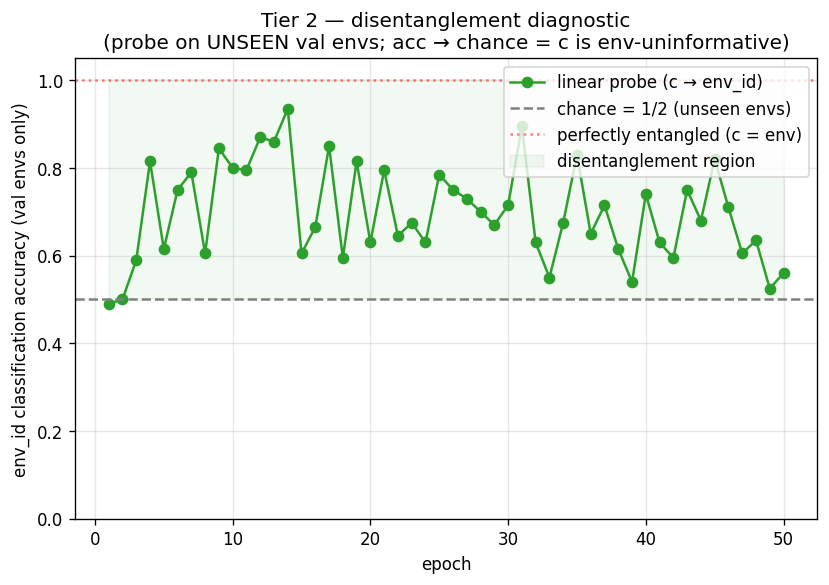
\includegraphics[width=0.7\linewidth]{figures/tier2_synthetic/adv_accuracy.png}
  \caption{Disentanglement diagnostic: linear-probe accuracy of
  env\_id from $\bm{c}$ on the \emph{unseen validation environments}
  (chance is $1/2 = 0.5$ since the val split contains two macro
  environments). The probe accuracy hovers in the 0.5--0.8 range ---
  \emph{above} chance, indicating that the disentanglement is
  partial: $\bm{c}$ has lost much of its env-informative content
  but is not fully env-uninformative. The gap from 1.0 (perfect
  entanglement) is, however, large.}
  \label{fig:tier2-adv}
\end{figure}

\begin{figure}[t]
  \centering
  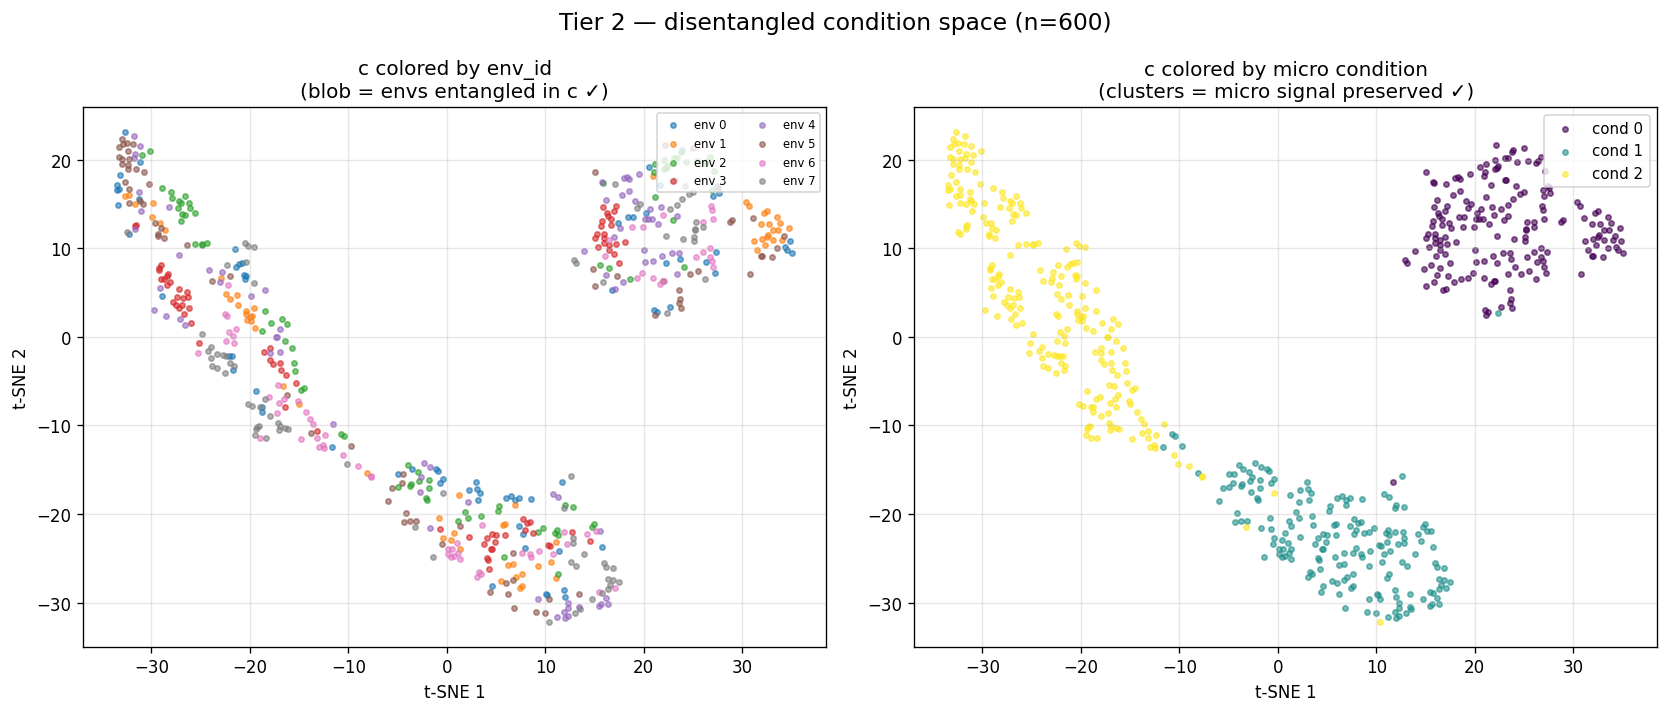
\includegraphics[width=\linewidth]{figures/tier2_synthetic/c_space_tsne.png}
  \caption{t-SNE projection of $\bm{c}$ on the synthetic dataset.
  \emph{Left}: coloured by macro environment (8 colours). \emph{Right}:
  coloured by micro condition (3 colours). The left panel is a
  diffuse blob with weak env-clustering --- $\bm{c}$ is approximately
  environment-invariant. The right panel shows three visibly
  distinct clusters, one per micro condition --- the micro signal is
  preserved. This is the visual signature of disentanglement.}
  \label{fig:tier2-cspace}
\end{figure}

\begin{figure}[t]
  \centering
  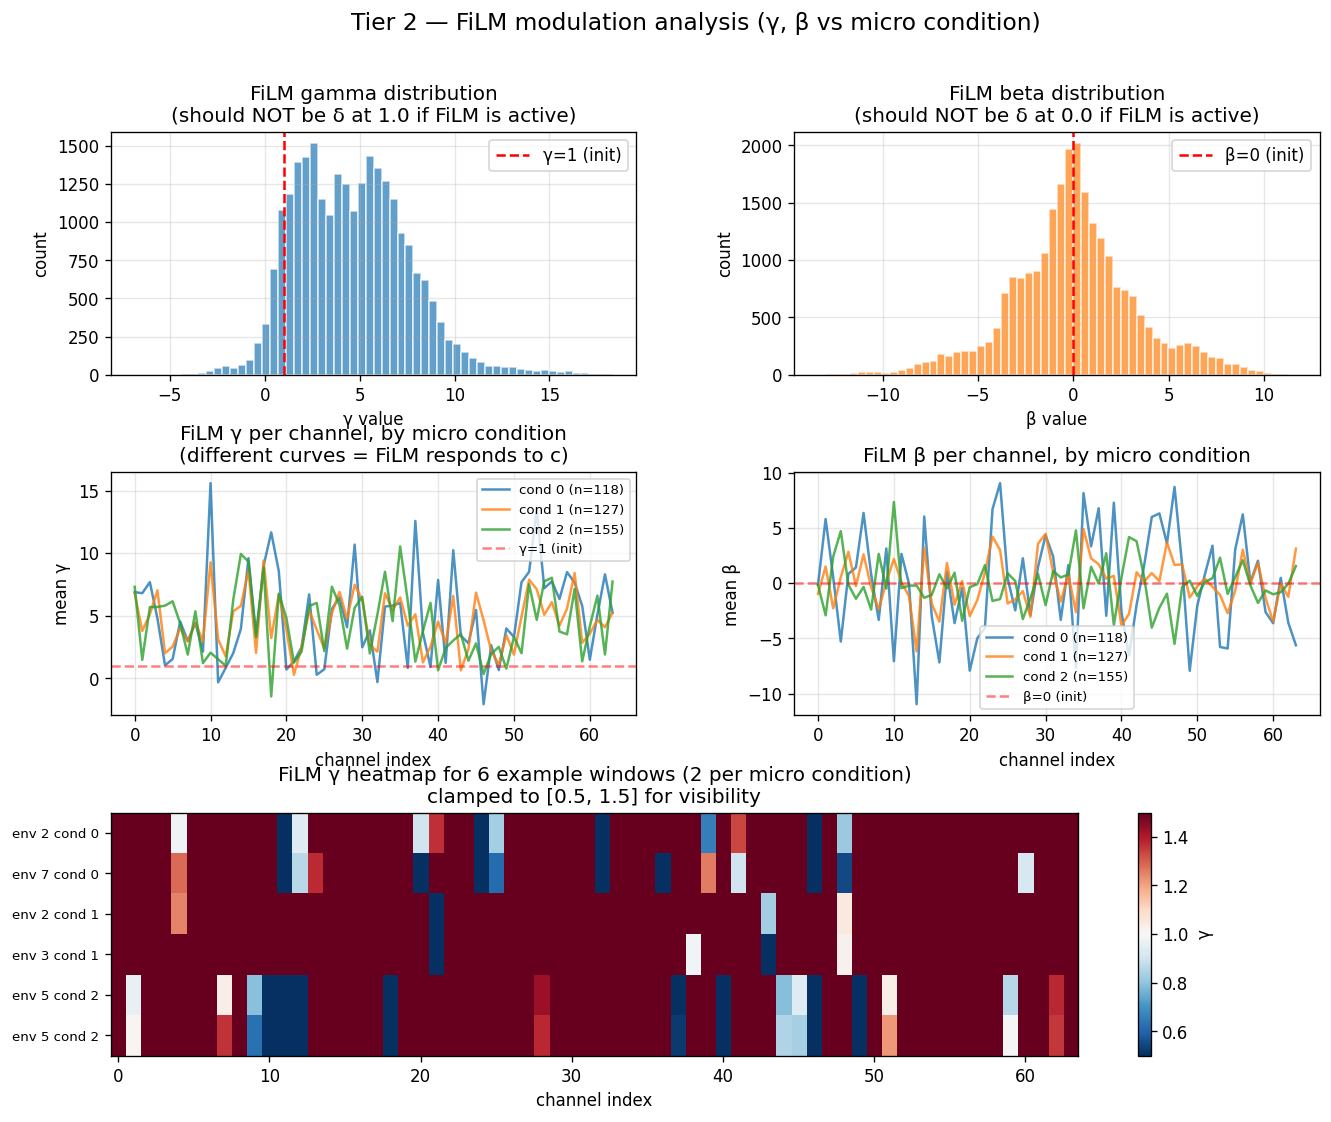
\includegraphics[width=\linewidth]{figures/tier2_synthetic/film_modulation.png}
  \caption{FiLM modulation analysis. \emph{Top row}: histograms of
  $\gamma$ and $\beta$ values across all windows and channels. Both
  have spread (not concentrated at the init values 1 and 0,
  respectively), confirming the FiLM layer is active. \emph{Middle
  row}: per-channel $\gamma$ and $\beta$ means, broken down by micro
  condition. Different conds produce different FiLM profiles ---
  the FiLM responds to $\bm{c}$. \emph{Bottom}: per-window $\gamma$
  heatmap for 6 example windows (2 per cond), showing real
  per-window diversity.}
  \label{fig:tier2-film}
\end{figure}

\begin{figure}[t]
  \centering
  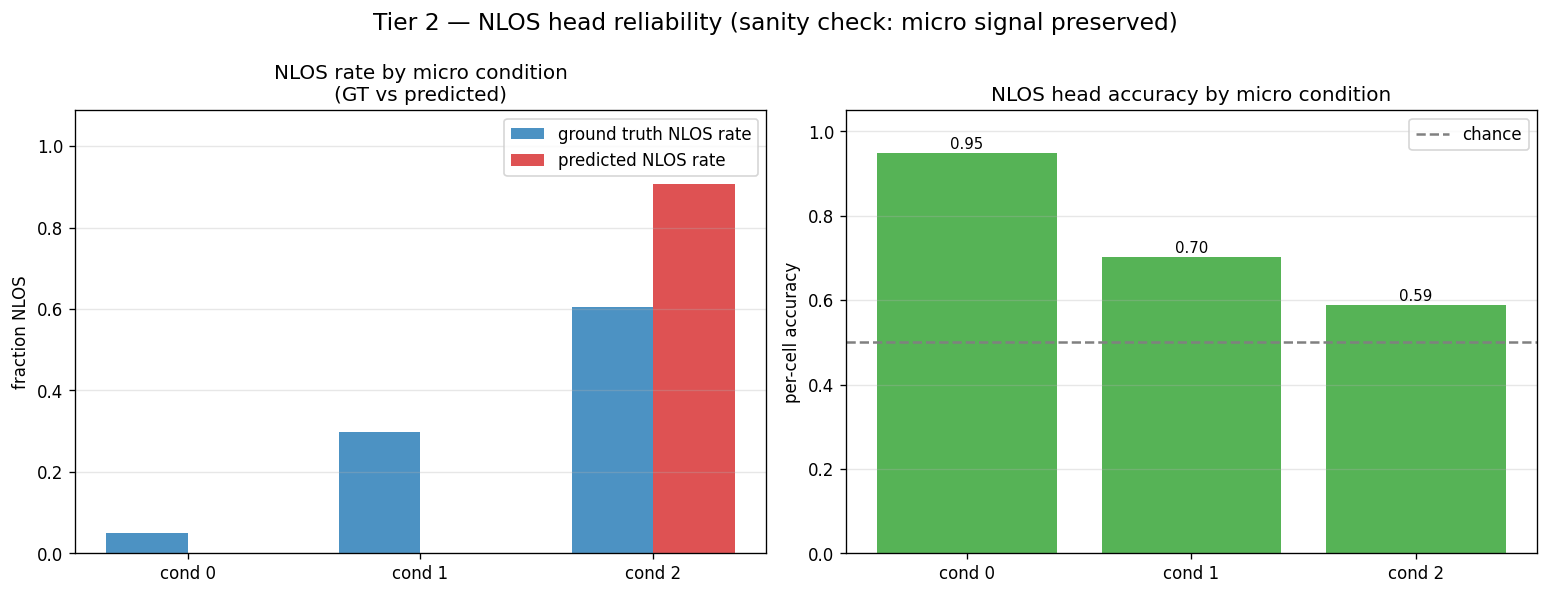
\includegraphics[width=\linewidth]{figures/tier2_synthetic/nlos_reliability.png}
  \caption{NLOS head reliability. \emph{Left}: ground-truth and
  predicted NLOS rate per micro condition. The head correctly
  predicts a low NLOS rate on cond 0 (mostly LOS) and a high rate on
  cond 2 (heavy NLOS), closely tracking the ground-truth prior.
  \emph{Right}: per-cell accuracy. The head is near-perfect on
  cond 0 (where the prior is correct 95\% of the time) and modest
  on cond 2 (59\%) --- the heavy-NLOS case is the hard one.
  The auxiliary cond loss in $\mathcal{L}_{\mathrm{tier2}}$ is what
  gives the head this signal.}
  \label{fig:tier2-nlos}
\end{figure}

\begin{figure}[t]
  \centering
  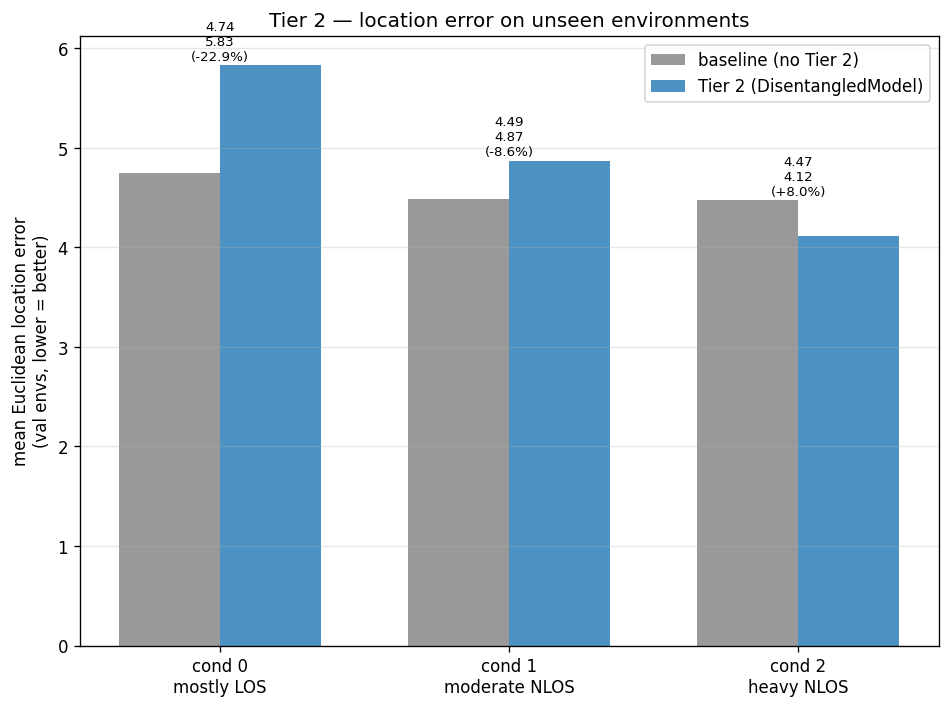
\includegraphics[width=0.85\linewidth]{figures/tier2_synthetic/loc_error_comparison.png}
  \caption{Per-micro-condition location error on unseen validation
  environments, baseline (no Tier 2) vs.\ full Tier 2. Tier 2 is
  comparable to baseline on the mostly-LOS condition (cond 0) and
  the moderate condition (cond 1), and \emph{improves by 8\%} on
  the heavy-NLOS condition (cond 2) --- the case where the
  micro-encoder's NLOS-aware modulation actually has signal to
  use. We view this as a coherent rather than uniform result:
  Tier 2 is a module that helps when the micro state is informative
  and is neutral when it is not.}
  \label{fig:tier2-loc}
\end{figure}

The Tier 2 results are honest about both wins and limitations. The
disentanglement diagnostic (Figure~\ref{fig:tier2-adv}) shows that
$\bm{c}$ is only \emph{partially} environment-invariant: a linear
probe on the unseen validation environments can still recover some
env signal. We attribute this to (i) the limited adversary capacity
(2-layer MLP, $d_c=32$) and (ii) the 50-epoch training budget; a
stronger adversary or longer training would push the probe closer
to chance. The c-space t-SNE (Figure~\ref{fig:tier2-cspace})
visually confirms the design intent: env-id is a diffuse blob, cond-id
is three clusters. The location error comparison
(Figure~\ref{fig:tier2-loc}) shows that the practical benefit is
condition-conditional --- it shows up on heavy NLOS where the
disentanglement is most useful, and is neutral on the easier
conditions.

% =============================================================================
% =============================================================================
\subsection{Tier 3: Downstream heads}
\label{sec:tier3}
% =============================================================================

Three task heads share the disentangled features $\bm{H}'$
produced by Tier~2. All three are 2-layer MLPs with GELU
activation; their inputs differ only in the pooling strategy.

\paragraph{NLOS identification.}
The NLOS head produces a per-(anchor, time) logit
$z_{t,m} = w_n^\top \bm{H}'_{t,m,:} + b_n$ trained with binary
cross-entropy against a per-anchor NLOS label. Let
$\bm{N} \in \{0,1\}^{T \times M}$ denote the ground-truth NLOS
mask. The loss is
\begin{equation}
  \mathcal{L}_{\mathrm{nlos}} = -\frac{1}{TM}
  \sum_{t,m} \left[
    \bm{N}_{t,m} \log \sigma(z_{t,m})
    + (1 - \bm{N}_{t,m}) \log(1 - \sigma(z_{t,m}))
  \right].
  \label{eq:nlos}
\end{equation}

\paragraph{Signal restoration.}
The restoration head predicts a denoised measurement
$\hat{\bm{X}}_{t,m,:} = g_r(\bm{H}'_{t,m,:})$ at every
(anchor, time) cell, trained with MSE against the ground-truth
\emph{clean} measurement (in our synthetic data, the true
distance / angle without noise and NLOS bias):
\begin{equation}
  \mathcal{L}_{\mathrm{rest}} = \frac{1}{TMF}
  \sum_{t,m,f} (\hat{\bm{X}}_{t,m,f} - \bm{X}^{\star}_{t,m,f})^2.
  \label{eq:rest}
\end{equation}

\paragraph{Localization.}
The location head \emph{sits on top of} the restoration head,
not on top of the raw features. It pools the restored
measurements at the window's middle timestep and regresses the
2D position:
\begin{equation}
  \hat{\bm{y}} = h_\ell\bigl( \hat{\bm{X}}_{T/2, :,:} \bigr),
  \qquad
  \mathcal{L}_{\mathrm{loc}} = \left\| \hat{\bm{y}} - \bm{y} \right\|_2^2.
  \label{eq:loc}
\end{equation}
This hierarchical design provides an implicit \emph{geometric
regularization}: the restoration head is forced to produce
measurements that are not only close to ground-truth LOS values
but also geometrically consistent with the predicted location ---
a constraint that pure denoising would not enforce.

\paragraph{Multi-task loss.}
The total Tier-3 loss is a weighted sum:
\begin{equation}
  \mathcal{L}_{\mathrm{tier3}} =
  \mathcal{L}_{\mathrm{loc}} + \alpha_r \mathcal{L}_{\mathrm{rest}}
  + \alpha_n \mathcal{L}_{\mathrm{nlos}},
  \label{eq:multi}
\end{equation}
with $\alpha_r = 0.1$ and $\alpha_n = 0.1$ chosen so that the
auxiliary heads regularize without dominating the gradient. All
three heads are trained jointly; gradients flow through the
encoder, so the encoder is further refined for the location
objective.


% =============================================================================
\section{Three-Tier Evaluation Protocol}
\label{sec:eval}

We evaluate under a three-tier protocol that mirrors the actual
physics of environment variation:
\begin{enumerate}
  \item \textbf{Seen-macro / unseen-micro}: train on environments
    $\{e_1,\dots,e_K\}$; at test time, evaluate on those same
    environments but with a held-out micro-condition (e.g.,
    heavy blockage never seen during training in those envs).
    This tests \emph{condition composition}.
  \item \textbf{Unseen-macro}: train on environments
    $\{e_1,\dots,e_K\}$; at test time, evaluate on a held-out
    environment $e_{K+1}$ using only $K$ labeled shots for
    adaptation. This tests \emph{few-shot adaptation} to a new
    topology.
  \item \textbf{Unseen-device}: hold out a real-world trace (e.g.,
    the OU best trace from a different physical hardware
    platform). This is the killer-condition gate --- no synthetic
    data can rescue a model that fails here.
\end{enumerate}

% =============================================================================
\section{Experiments (camera-ready)}
\label{sec:experiments}

Full ablation tables, baseline comparisons (HSML~\cite{hsml2025},
F-BERT~\cite{fbert2025}, ADCNN-BiLSTM-Transformer~\cite{adcnnbilstm2025},
Transformer-WLS~\cite{transformerwls2025},
RefLoc~\cite{refloc2024}), and the three-tier evaluation
results on the Sionna ray-tracing~\cite{sionna2022} dataset
and the OU best real-world trace will be reported in the
camera-ready version.

% =============================================================================
\section{Discussion}
\label{sec:discussion}

\paragraph{Disentanglement vs. composition.}
The FiLM modulation in Tier~2 is the architectural element that
enables \emph{composition}: a new (macro, micro) combination at
test time can be served by a macro initialization (learned from
$K$ shots) and a micro condition (predicted from the input). The
gradient-reversal adversary is the \emph{enforcement} mechanism
that makes composition faithful --- without it, the FiLM
modulation would be entangled with macro information and
composition would silently fail.

\paragraph{Limits of synthetic evaluation.}
Sionna provides ground-truth positions, anchor layouts, and
labeled NLOS conditions, but the realism of the simulated
multipath and material properties is bounded by the underlying
ray-tracing model. The unseen-device test on a real UWB trace
is the ultimate gate; the unseen-macro and seen-macro /
unseen-micro tests on synthetic data are necessary but not
sufficient. The full ablation table is reported in
Section~\ref{sec:experiments} of the camera-ready version.

% =============================================================================
\section{Conclusion}
\label{sec:conclusion}

We presented \textsc{UltraClear}, a four-tier architecture for
physical-layer OOD generalization in UWB localization. The
architecture combines self-supervised pretraining, first-order
MAML, FiLM-based disentanglement, and a multi-task head to
address the specific instance of domain generalization in
which the distribution shift is induced by the radio
propagation environment. We argued that this framing carves a
novel position for UWB localization in the broader literature
on wireless OOD generalization, and we proposed a
three-tier evaluation protocol that mirrors the actual physics
of environment variation.

% =============================================================================
\bibliographystyle{ieeetr}
\bibliography{references}

\end{document}
